\chapter{Visualization on the Web}
\label{chap:visuzlization_web}

\begin{figure}[ht]
	\hfill
	\begin{minipage}{0.5\textwidth}
		\centering
		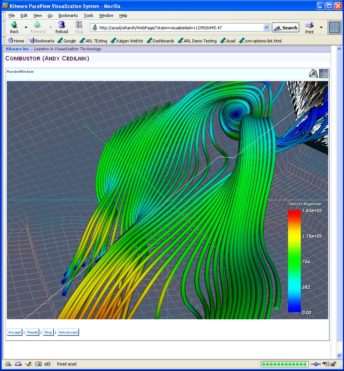
\includegraphics{VTKTextbook-269}
		\caption*{\texttt{Streamline visualization with ParaView Enterprise Edition.}}
	\end{minipage}
\end{figure}


\firstletter{T}he early 1990s established the widespread use and accessibility of the World Wide Web.
Once a network used primarily by researchers and universities, the Web has become something that is used by people throughout the world.
The effects of this transformation have been significant, ranging from personal home pages with static images and text, to professional Web pages embedding animation and virtual reality.
This chapter discusses some of those changes and describes how the World Wide Web can be used to make visualization more accessible, interactive, and powerful.
Topics covered include the advantages and disadvantages of client-side versus server-side visualization, VRML, and Java3D, interwoven with demonstration examples.

\section{Motivation}
Before describing in detail how to perform visualization over the Web, it is important to understand what we expect to gain. Clearly people have been visualizing data prior to the invention of the Web, but what the Web adds is the ability for people throughout the world to share information quickly and efficiently.
Like all successful communication systems, the Web enables people to interact and share information more efficiently compared to other methods.
In many ways the Web shares the characteristic of computer visualization in its ability to communicate large amounts of data.
For that reason, computer graphics and visualization are now vital parts of the Web, and are becoming widespread in their application.
